\subsection{UAS Movement Automaton}\label{s:movementAutomatonDefinition}

\paragraph{Motivation:} An \emph{UAS Nonlinear Model} (eq. \ref{eq:UASNonlinearModelSimple}) can be modeled by \emph{Movement Automaton} (def. \ref{def:movementAutomaton}). 

\paragraph{Movement Primitives} by (def. \ref{def:MovementPrimitive})  are given as (eq. \ref{eq:movementPrimitive}). Each movement primitive will last for fixed duration $1s$.
 

\begin{assumption}\label{ass:transitionTime}
    Let assume that \emph{transition time} of \emph{roll, pitch, yaw, and the linear velocity} is $0 s$.
\end{assumption}

Under the assumption (as. \ref{ass:transitionTime}) the \emph{movement transitions} (def. \ref{def:movementTransition}) have zero duration. Therefore movement primitives can be considered as movements.

\begin{note}
    The assumption (as. \ref{ass:transitionTime}) can be relaxed under the condition that \emph{path tracking controller exists}.
\end{note}

\paragraph{Movements} satisfying (def. \ref{def:Movement}), for the nonlinear model (eq. \ref{eq:UASNonlinearModelSimple}) reduced to \emph{discrete model} (eq. \ref{eq:uasLinearDiscreteModel}), are given by \emph{apply movements} function (eq. \ref{eq:applyMovement}, \ref{eq:applyMovement1}, \ref{eq:applyMovement2}).

\begin{equation}\label{eq:uasLinearDiscreteModel}
    state(k+1) = applyMovement(state(k), input(k)) 
\end{equation}

\paragraph{Movement Set} for the discrete model (eq. \ref{eq:uasLinearDiscreteModel}) is defined as a set of unitary movements on main axes (tab. \ref{tab:movements1}) and diagonal axes (tab. \ref{tab:movements2}). 

The maneuvering capability of several commercial small fixed-wing UAS was abstracted together. The turning rate on horizontal/vertical is defined as $15^\circ$.

The deltas are posed in \emph{UAS body-fixed coordinate frame} (ap. \ref{sec:complementsOfAlgebra}) for discrete time $k$. 

\begin{table}[H]
    \centering
    \begin{tabular}{r||r|r|r|r|r}
    	\multirow{2}{*}{Parameter} & \multicolumn{5}{c}{Movement} \\\cline{2-6} 
                &    Straight  & Down & Up & Left  & Right   \\\hline\hline
        $\delta     x(k)[m]$           &    1.00	  & 0.98  & 0.98  & 0.98 & 0.98  \\\hline
        $\delta     y(k)[m]$           &    0	      & 0	  & 0	  & 0.13 & -0.13 \\\hline
        $\delta     z(k)[m]$           &    0	      & -0.13 & 0.13  &	0	 & 0     \\\hline
        $\delta  roll(k) [^\circ]$	   &    0	      & 0	  & 0	  & 0    & 0     \\\hline
        $\delta pitch(k) [^\circ]$     &    0	      & $15^\circ$  & -$15^\circ$ & 0	 & 0     \\\hline
        $\delta   yaw(k) [^\circ]$     &    0	      & 0	  & 0	  & $15^\circ$ & -$15^\circ$ \\
    \end{tabular}
    \caption{Input values for main axes movements.}
    \label{tab:movements1}
\end{table}
\begin{table}[H]
    \centering
    \begin{tabular}{r||r|r|r|r}
    	\multirow{2}{*}{Parameter} & \multicolumn{4}{c}{Movement} \\\cline{2-5} 
                    & Down-Left & Down-Right & Up-Left  & Up-Right   \\\hline\hline
        $\delta     x(k)[m]$           & 0.76  & 0.76  & 0.76 & 0.76  \\\hline
        $\delta     y(k)[m]$           & -0.13	& 0.13	& 0.13 & -0.13 \\\hline
        $\delta     z(k)[m]$           & -0.13 & -0.13 & 0.13 & 0.13  \\\hline
        $\delta  roll(k) [^\circ]$	& 0	    & 0	    & 0    & 0     \\\hline
        $\delta pitch(k) [^\circ]$     & -$15^\circ$ & -$15^\circ$ & $15^\circ$ & $15^\circ$     \\\hline
        $\delta   yaw(k) [^\circ]$    & $15^\circ$	& -$15^\circ$	& $15^\circ$ & -$15^\circ$ \\
    \end{tabular}
    \caption{Input values for diagonal axes movements.}
    \label{tab:movements2}
\end{table}

\begin{note}
    The \emph{movement set} in shortened form is given as:
    \begin{equation}\label{eq:OurMovementSet}
        Movement Set= \left\{
        \begin{gathered}
            Straight, Left,Right, Up, Down,\\
            Down Left, Down Right,  Up Left,   Up Right
        \end{gathered}
        \right\}
    \end{equation}
\end{note}

The \emph{implemented movement set example} (fig. \ref{fig:implementedMovementSetExample}) shows the movement used as basic building blocs of the trajectory for fixed-wing UAS:
\begin{enumerate}
    \item \emph{Initial position} (red plane) - the initial position, before any movement execution.
    
    \item \emph{Straight movement application} (blue plane) - the \emph{neutral movement application} brings plane forward. 
    
    \item \emph{Main axes movements} (cyan planes) - the application of movements from (tab. \ref{tab:movements1}) $\{Up,$ $Down,$ $Left,$ $Right\}$.
    
    \item \emph{Diagonal axes movements} (magenta planes) - the application of movements from (tab. \ref{tab:movements2}) $\{Down Left,$ $Down Right,$  $Up Left,$   $Up Right\}$.
 \end{enumerate}
\begin{figure}[H]
    \centering
    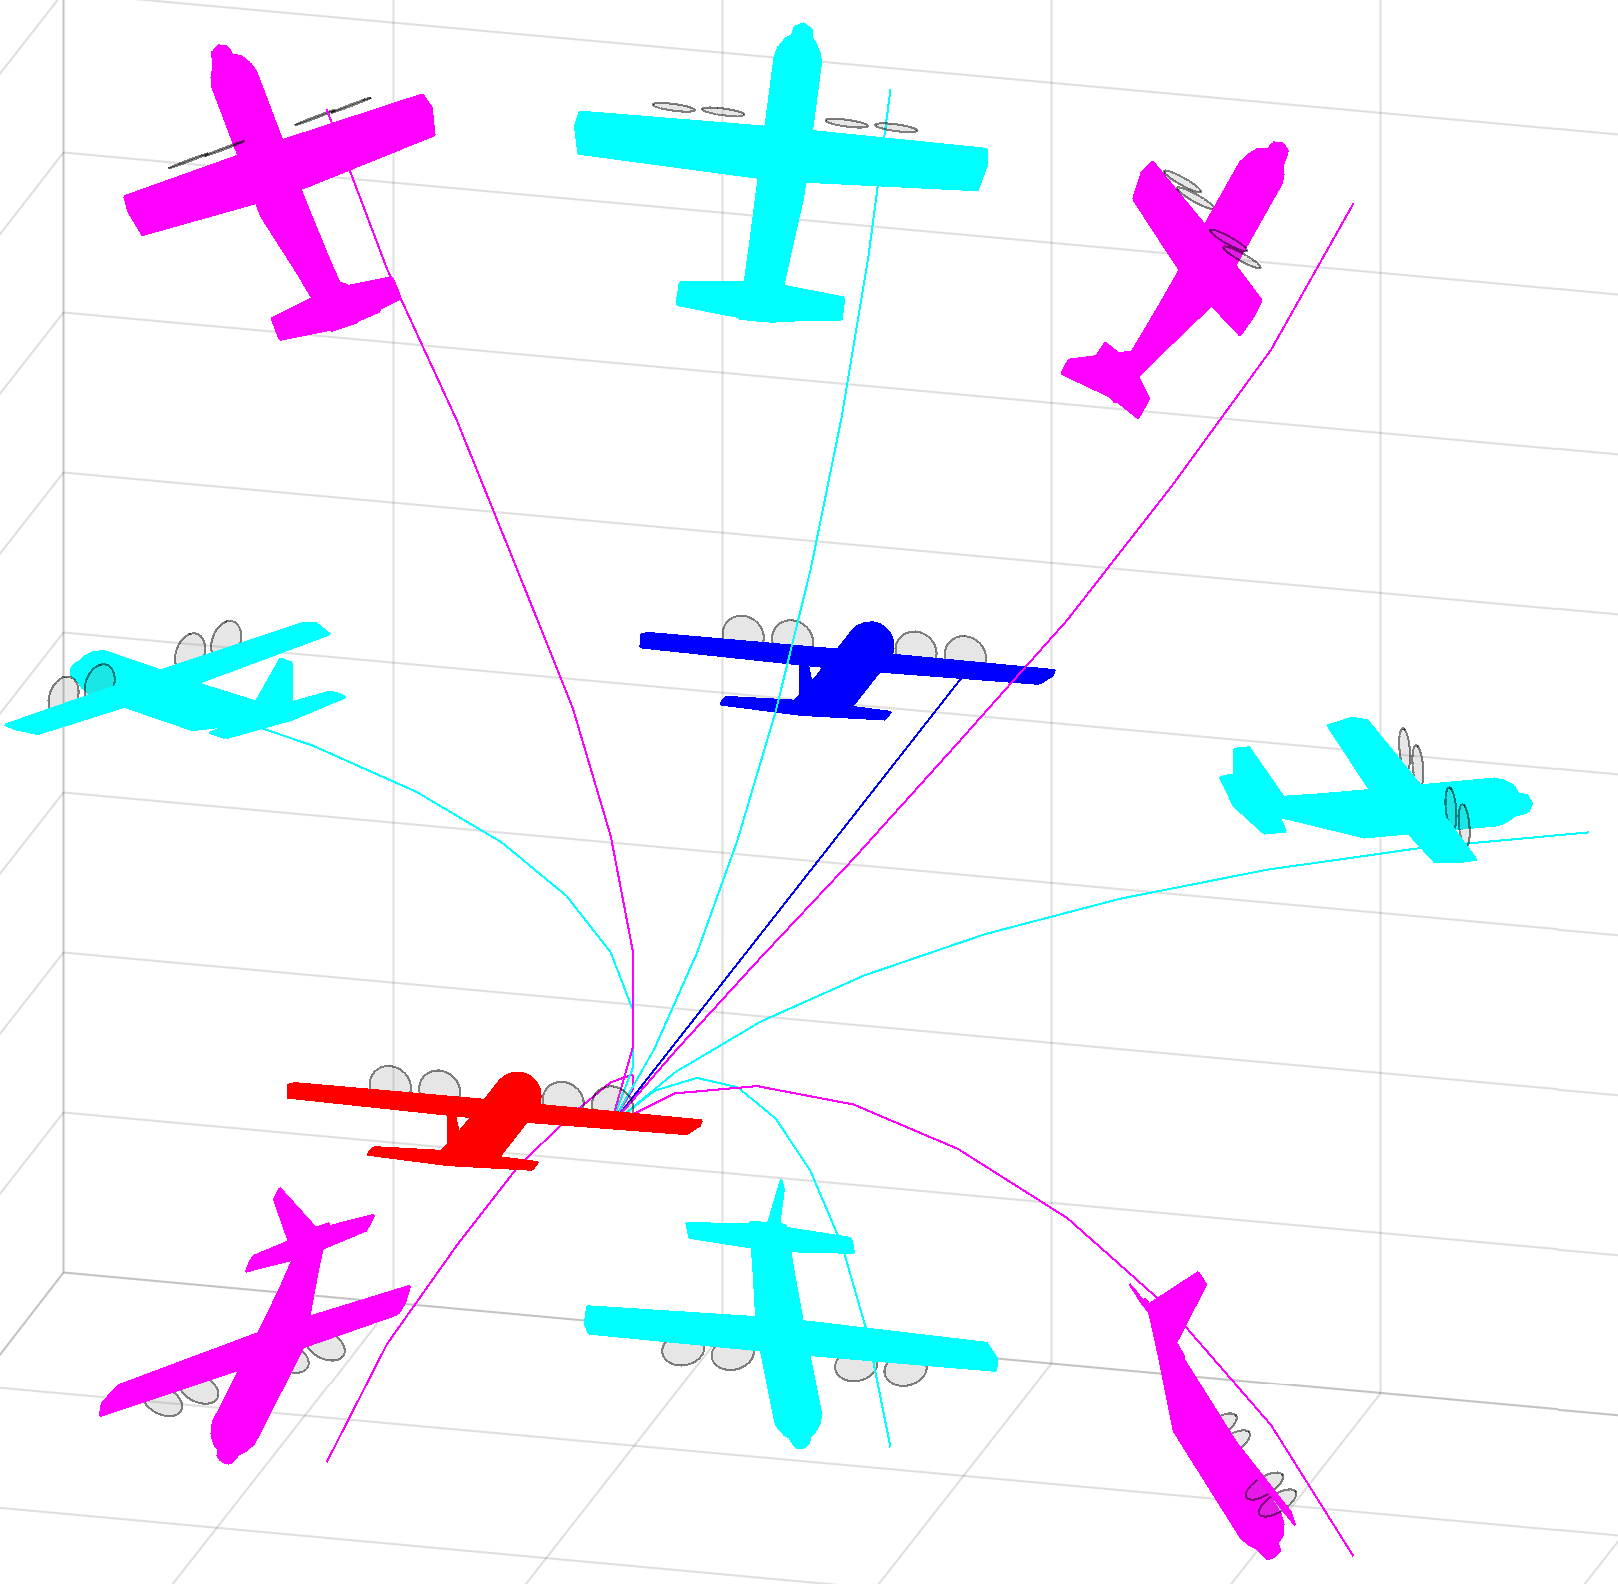
\includegraphics[width=0.55\textwidth]{\FIGDIR/TE065MovementSet}
    \caption{Implemented movement set example.}
    \label{fig:implementedMovementSetExample}
\end{figure}

\paragraph{Trajectory} by (def. \ref{def:MovementAutomatonTrajectory}) for initial time $time = 0$ , initial state $state(0)$ and \emph{Movement Buffer} (from def. \ref{def:MovementBuffer}):
\begin{equation}\label{eq:ourBuffer}
    Buffer = \left\{
                movement(j):
                \begin{aligned}
                    &movement(j)\in Movement Set (eq. \ref{eq:OurMovementSet}),\\
                    & j \in 1\dots n, n \in N^+
                \end{aligned}
            \right\}
\end{equation}

\begin{assumption}
    The buffer is always non-empty, ordered, finite list of \emph{movements}.
\end{assumption}

\begin{note}
  The buffer has finite count $n$ of movements stored. The buffer is the planning instrument used by higher level navigation/avoidance algorithm to control UAS (Control/Command interface) (fig. \ref{fig:AvoidanceFrameworkConceptNew}).
\end{note}

%\noindent Trajectory (eq. \ref{eq:ourTrajectoryImplementation}) is then %given as the time-series of discrete states:
%\begin{equation}\label{eq:ourTrajectoryImplementation}
%    Trajectory(state(0),Buffer)= \left\{\begin{gathered}state(0)+\sum_{j=0}%^{i-1} input(movement(j)):\\i \in\left\{1\dots |Buffer|+1\right\}, \%\movement(\cdot) \in Buffer\end{gathered}\right\}
%\end{equation}

The discrete trajectory (eq. \ref{eq:ourTrajectoryEvolution}) is ordered set of states bounded to discrete time $0\dots n$, where $n$ is movement count of \emph{Buffer}. Trajectory set has $n+1$ members defined like the following:

\begin{equation}\label{eq:ourTrajectoryEvolution}
    \begin{aligned}
    T&rajectory(state(0),Buffer)=\\
        &\left\{
        \begin{aligned}
            state(0) &= state(0),\\
            state(1) &= apply Movement\left(state(0), movement(1)\right),  \\
            state(2) &= apply Movement\left(state(1), movement(2)\right),  \\
             \vdots  &= \vdots\\
            state(n-1) &= apply Movement\left(state(n-2), movement(n-1)\right),  \\
            state(n)   &= apply Movement\left(state(n-1), movement(n)\right)  \\
        \end{aligned}
        \right\}
    \end{aligned}
\end{equation}

\noindent The movement$(k)$ vector is selected from movement tables (tab. \ref{tab:movements1}, \ref{tab:movements2}).

\begin{note}
	Parameter movement($\cdot$) (eq. \ref{eq:ourTrajectoryEvolution}) is a movement order index in buffer (eq. \ref{eq:ourBuffer}).
\end{note}